\documentclass{beamer}

\usepackage{mathpazo}
\usetheme{Warsaw} % Tema escogido en este ejemplo
\usepackage[latin1]{inputenc}
\usepackage{latexsym} 
\usepackage{amsmath}
\usepackage{amssymb}

\author[]{jltabara@gmail.com}
\title[]{Teor�a de grafos con Algraf}
\date{}

\begin{document}

\frame{\titlepage}





\begin{frame}{Grafos I. Construcci�n}



\begin{figure}
\begin{minipage}{0.60 \textwidth}

\begin{itemize}

\item  Crea un grafo similar al de la imagen.


\item Mueve sus v�rtices y ren�mbralos.



\item Calcula los grados de los v�rtices y comprueba la f�rmula de la suma de los grados.

\item  Construye la matriz de adyacencias e interpr�tala.

\item Guarda una imagen del grafo.

\item  Guarda el grafo.

\item Borrar aristas y v�rtices para construir subgrafos.


\end{itemize}

\end{minipage}
\   \
\hfill \begin{minipage}{ 3.5cm}% Tambi�n se puede indicar en cms

\begin{center}
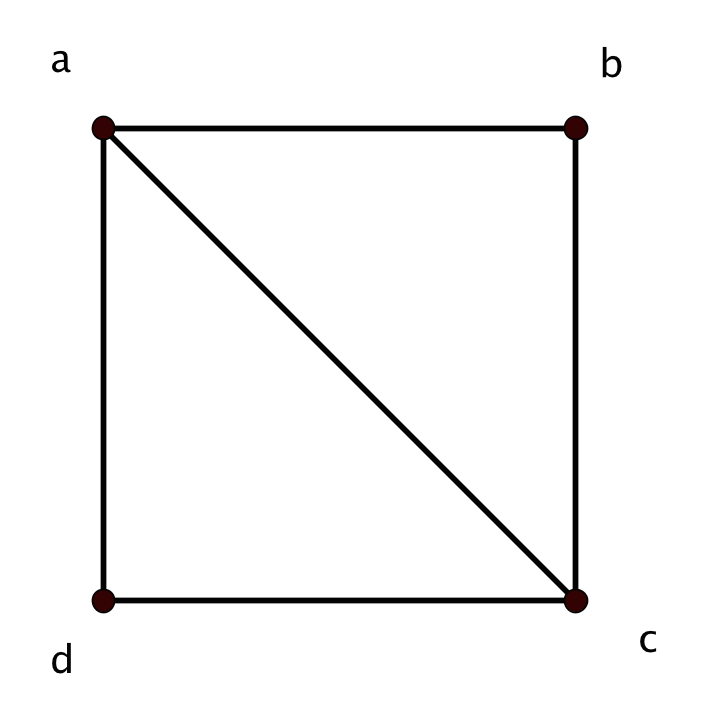
\includegraphics[width=3.5cm]{grafo01.png}
\end{center}


\end{minipage}

\end{figure}

\end{frame}

\begin{frame}{Grafos II. Conexi�n}



\begin{itemize}

\item  Encuentra un camino entre dos v�rtices de un grafo conexo.

\item Comprueba que si algunos v�rtices no se pueden unir por un camino, el grafo no es conexo (tiene m�s de una componente conexa).

\item Encuentra el n�mero de componentes conexas de un grafo.

\item Encuentra aristas puente. Comprueba que al eliminar una arista puente el grafo tiene m�s componentes conexas.

\item Encuentra los puntos de corte y comprueba que su eliminaci�n aumenta el n�mero de componentes conexas.




\end{itemize}

\end{frame}

\begin{frame}{Grafos III. Algunos grafos famosos}



\begin{itemize}

\item  Construir el grafo completo $K_5$ y analizar su matriz.

\item Construir el grafo bipartito completo $K_{3,4}$ y analizar su matriz.

\item Construir el grafo plat�nico del octaedro y analizar su matriz.

\item Construir el grafo complementario y analizar su matriz.

\item Construir el complementario del complementario.

\item  Construir un grafo simple a partir de su matriz.




\end{itemize}

\end{frame}


\begin{frame}{Grafos IV. Grafos isomorfos}



\begin{itemize}

\item Dos grafos isomorfos deben tener el mismo n�mero de v�rtices, de aristas, de componentes conexas y la sucesi�n de sus grados debe ser igual.

\item Comprobar, mediante un ejemplo, que las condiciones anteriores son necesarias, pero no suficientes para que sean isomorfos.


\item Si dos grafos son isomorfos, sus complementarios tambi�n lo son.


\item Analizar las matrices de dos grafos isomorfos.


\end{itemize}

\end{frame}


\begin{frame}{Grafos V. Grafos eulerianos}


\begin{itemize}

\item Ejemplo de grafo no euleriano.


\item Ejemplo de grafo semieuleriano y trazado de un camino con el algoritmo de Fleury.


\item Construcci�n de un ciclo euleriano por parte del usuario.


\item M�todo para convertir en euleriano y grafo con dos v�rtices de grado impar (semieuleriano).


\end{itemize}

\end{frame}


\begin{frame}{Grafos VI. Sucesiones gr�ficas}



\begin{itemize}

\item C�lculo de la sucesi�n gr�fica de un grafo con el programa Petersen.


\item Construcci�n de la sucesi�n gr�fica $\{6,5,2,2,2,2,1\}$.


\item Construcci�n de la sucesi�n gr�fica $\{0,1,2,2,3\}$.

\item Construcci�n de la sucesi�n gr�fica $\{2,2,4,4,4\}$


\item La p�gina para la descarga del programa Petersen es:

\begin{center}
{\scriptsize\texttt{www.mathcove.net/petersen/lessons/getting-petersen?les=0}}
\end{center}

\end{itemize}

\end{frame}



\end{document}





























